\documentclass[11pt,a4paper]{article}

% ==============================================================================
% EXPERIMENT 06: PRINTABLE SOURCE CODE & OUTPUT (EXACT SINGLE 1-PAGE DOCUMENT)
% Formatted with 1.0-inch lateral margins, large readable fonts, and tight top/bottom margins.
% ==============================================================================
\usepackage[utf8]{inputenc}
\usepackage[T1]{fontenc}
\usepackage{lmodern}
\usepackage[left=1.0in, right=1.0in, top=0.32in, bottom=0.32in]{geometry}
\usepackage{amsmath,amssymb}
\usepackage{xcolor}
\usepackage{listings}
\usepackage{tikz}
\usetikzlibrary{arrows.meta,positioning,calc}
\usepackage{booktabs}
\usepackage{tabularx}
\usepackage{titlesec}
\usepackage{caption}
\usepackage{microtype}
\usepackage{float}

% Disable all running headers, footers, and page numbers for clean print & paste
\pagestyle{empty}
\setlength{\parindent}{0pt}

% Section Titles Formatting (Enlarged)
\titleformat{\section}
  {\normalfont\large\bfseries\raggedright}{\thesection}{0.6em}{}[\titlerule]

\titlespacing*{\section}{0pt}{5pt}{2pt}

% Code Listing Styling (Strict Monochrome with Enlarged Font for High-Contrast Print)
\lstdefinestyle{bwArduino}{
    language=C++,
    basicstyle=\ttfamily\footnotesize,
    keywordstyle=\bfseries,
    commentstyle=\itshape,
    stringstyle=\ttfamily,
    numbers=left,
    numberstyle=\tiny,
    numbersep=6pt,
    stepnumber=1,
    breaklines=true,
    breakatwhitespace=true,
    frame=single,
    rulecolor=\color{black},
    tabsize=2,
    showstringspaces=false,
    columns=fullflexible,
    keepspaces=true,
    lineskip=-0.1pt,
    aboveskip=2pt,
    belowskip=2pt
}

\lstdefinestyle{bwTerminal}{
    basicstyle=\ttfamily\footnotesize,
    numbers=none,
    breaklines=true,
    breakatwhitespace=true,
    frame=single,
    rulecolor=\color{black},
    columns=fullflexible,
    keepspaces=true,
    lineskip=1.2pt,
    aboveskip=2pt,
    belowskip=2pt
}

\captionsetup{font=small,labelfont=bf,skip=2pt}

\begin{document}

% ==============================================================================
% DOCUMENT HEADER
% ==============================================================================
\begin{center}
    {\large\bfseries Experiment 06: Interfacing PIR Motion Sensor with Arduino UNO}\\[0.08cm]
    {\normalsize\textbf{Passive Infrared Motion Detection \& Alert Telemetry --- Program Source Code \& Experimental Output}}
\end{center}
\vspace{-0.20cm}
\rule{\textwidth}{0.9pt}
\vspace{0.06cm}

% ==============================================================================
% 1. PROGRAM SOURCE CODE
% ==============================================================================
\section*{1. Arduino C++ Source Code}

\begin{lstlisting}[style=bwArduino, title={\textbf{Listing 6.1: Microcontroller Firmware for PIR Motion Sensing and Serial Event Telemetry.}}]
/*
 * Experiment 06: PIR Motion Sensor Interfacing with Arduino UNO
 * Hardware Pin Connections:
 *   - PIR Sensor OUT (O/P) -> Arduino Digital Pin 8 (Configured as INPUT)
 *   - PIR Sensor VCC       -> Arduino 5V Power Rail
 *   - PIR Sensor GND       -> Arduino Common Ground (GND)
 * Serial Baud Rate: 9600 bps | Sampling Interval: 100 ms
 */

const int motionPin = 8; // Digital input pin connected to PIR OUT

void setup() {
  pinMode(motionPin, INPUT); // Configure Pin 8 as digital input
  Serial.begin(9600);        // Initialize UART Serial Interface at 9600 Baud
}

void loop() {
  // Acquire digital logic state from PIR pyroelectric sensor module
  if (digitalRead(motionPin) == HIGH) {
    Serial.println("motion detected!");
  } else {
    Serial.println("No motion");
  }
  delay(100); // 100 ms sampling cycle delay to prevent buffer saturation
}
\end{lstlisting}

\vspace{0.06cm}

% ==============================================================================
% 2. EXPERIMENTAL OUTPUT & LOGIC WAVEFORMS (SERIAL: 2.A -> 2.B -> 2.C)
% ==============================================================================
\section*{2. Experimental Output, Detection State Log \& Digital Waveforms}

\noindent
\textbf{A. Motion Detection Observation Log:}\par\vspace{0.06cm}
{\footnotesize
\setlength{\tabcolsep}{4.5pt}
\renewcommand{\arraystretch}{1.18}
\begin{tabularx}{\textwidth}{|c|p{4.6cm}|c|c|X|}
\hline
\textbf{\#} & \textbf{Human Target Motion State} & \textbf{Pin 8 Output} & \textbf{Serial Output} & \textbf{Hardware Alert Status} \\
\hline
1 & Quiescent / Idle Baseline & LOW ($0\,\text{V}$) & \texttt{No motion} & Quiescent Baseline (Sensor Armed) \\
2 & Active Hand Movement & HIGH ($5\,\text{V}$) & \textbf{\texttt{motion det.!}} & Motion Triggered ($T_{\text{hold}}$ Active) \\
3 & Continuous Motion Transit & HIGH ($5\,\text{V}$) & \textbf{\texttt{motion det.!}} & Retrigger Interval Extended \\
4 & Target Stationary State & LOW ($0\,\text{V}$) & \texttt{No motion} & Quiescent Baseline (Reset) \\
5 & Secondary Transit Cycle & HIGH ($5\,\text{V}$) & \textbf{\texttt{motion det.!}} & Motion Triggered ($T_{\text{hold}}$ Active) \\
\hline
\end{tabularx}
}

\vspace{0.20cm}

\noindent
\textbf{B. Serial Monitor Stream (9600 Baud):}\par\vspace{0.05cm}
\begin{lstlisting}[style=bwTerminal]
motion detected!
motion detected!
No motion
No motion
motion detected!
\end{lstlisting}

\vspace{0.18cm}

\noindent
\textbf{C. PIR Sensor Thermal Flux \& Digital Output Timing Waveform ($T_{\text{hold}}$):}\par\vspace{0.05cm}
{\centering
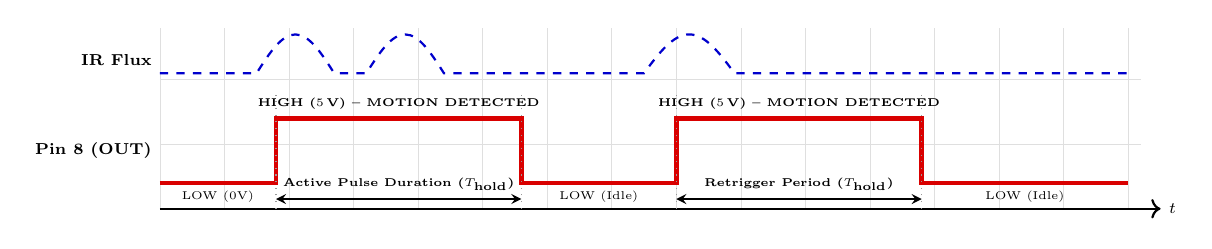
\begin{tikzpicture}[scale=0.82, every node/.style={transform shape}]
    \draw[step=1.0cm,gray!25,very thin] (0,0) grid (15.2,2.8);
    \draw[thick,->] (0,0) -- (15.5,0) node[right, font=\scriptsize] {$t$};
    
    % IR Heat Flux / Movement (Analogue stimulus)
    \draw[dashed, blue!80!black, thick] 
        (0,2.1) -- (1.5,2.1) 
        sin (2.1,2.7) cos (2.7,2.1) -- (3.2,2.1)
        sin (3.8,2.7) cos (4.4,2.1) -- (7.5,2.1)
        sin (8.2,2.7) cos (8.9,2.1) -- (15.0,2.1);
    \node[left, font=\scriptsize\bfseries] at (0,2.3) {IR Flux};

    % Digital Pin 8 Pulse (PIR Output)
    \draw[ultra thick, red!85!black] 
        (0,0.4) -- (1.8,0.4) -- (1.8,1.4) -- (5.6,1.4) -- (5.6,0.4) 
        -- (8.0,0.4) -- (8.0,1.4) -- (11.8,1.4) -- (11.8,0.4) -- (15.0,0.4);
    \node[left, font=\scriptsize\bfseries] at (0,0.9) {Pin 8 (OUT)};
    
    % Logic State labels
    \node[below, font=\tiny] at (0.9,0.4) {LOW (0V)};
    \node[above, font=\tiny\bfseries] at (3.7,1.42) {HIGH ($5\,\text{V}$) -- MOTION DETECTED};
    \node[below, font=\tiny] at (6.8,0.4) {LOW (Idle)};
    \node[above, font=\tiny\bfseries] at (9.9,1.42) {HIGH ($5\,\text{V}$) -- MOTION DETECTED};
    \node[below, font=\tiny] at (13.4,0.4) {LOW (Idle)};
    
    % Timing markers
    \draw[dotted, gray!80] (1.8,0) -- (1.8,1.8);
    \draw[dotted, gray!80] (5.6,0) -- (5.6,1.8);
    \draw[<->, >=stealth, black, semithick] (1.8,0.15) -- (5.6,0.15) node[midway, above, font=\tiny\bfseries] {Active Pulse Duration ($T_{\text{hold}}$)};
    
    \draw[dotted, gray!80] (8.0,0) -- (8.0,1.8);
    \draw[dotted, gray!80] (11.8,0) -- (11.8,1.8);
    \draw[<->, >=stealth, black, semithick] (8.0,0.15) -- (11.8,0.15) node[midway, above, font=\tiny\bfseries] {Retrigger Period ($T_{\text{hold}}$)};
\end{tikzpicture}\par\vspace{0.05cm}
{\small\textbf{Figure 6.1:} PIR sensor analog IR flux response and digital retrigger timing waveform ($T_{\text{hold}}$).}\par}

\end{document}
